\documentclass[final]{beamer}
\usepackage[size=a0,orientation=landscape,scale=0.93]{beamerposter}
\usepackage{graphicx}
\usepackage{amsmath,amssymb}
\usepackage{booktabs}
\usepackage{ragged2e}
\usepackage[T1]{fontenc}
\usepackage{lmodern}

\definecolor{DeepBlue}{HTML}{065A82}
\definecolor{Teal}{HTML}{1C7293}
\definecolor{Midnight}{HTML}{21295C}
\definecolor{LightGray}{HTML}{F2F2F2}

\setbeamercolor{headline}{fg=white,bg=Midnight}
\setbeamercolor{block title}{fg=white,bg=DeepBlue}
\setbeamercolor{block body}{fg=black,bg=white}
\setbeamercolor{block alerted title}{fg=white,bg=Teal}
\setbeamercolor{block alerted body}{fg=black,bg=LightGray}
\setbeamertemplate{navigation symbols}{}
\setbeamertemplate{caption}[numbered]
\setlength{\columnsep}{2.2cm}

\title{A Rate--Distortion View of Semantic Information}
\subtitle{Numerical Reproduction of Binary and Gaussian Case Studies}
\author{EE142 Information Theory Course Project}
\institute{ShanghaiTech University}

\newcommand{\sordf}{R(D_s,D_a)}
\newcommand{\figw}{0.82\linewidth}

\begin{document}
\begin{frame}[t]

\begin{beamercolorbox}[wd=\paperwidth,sep=1.0cm,center]{headline}
  {\Huge\bfseries \inserttitle}\par\vspace{0.10cm}
  {\Large \insertsubtitle}\par\vspace{0.08cm}
  {\large \insertauthor \quad | \quad \insertinstitute}
\end{beamercolorbox}

\vspace{0.35cm}
\begin{columns}[t,totalwidth=0.96\paperwidth]

\begin{column}{0.31\paperwidth}
\begin{block}{Semantic information is modeled as reconstructing both meaning and appearance}
\justifying
The paper represents an information source by a hidden semantic state $S$ and an observable appearance $X$. The encoder only observes $X$, but the decoder must reproduce both $\hat S$ and $\hat X$.
\[
\sordf = \min I(X;\hat S,\hat X)
\]
subject to semantic distortion $D_s$ and appearance distortion $D_a$.

\vspace{0.12cm}
\begin{itemize}
  \item $S$: intrinsic state or semantic content.
  \item $X$: extrinsic observation or appearance.
  \item $D_s$: task/meaning distortion.
  \item $D_a$: signal/appearance distortion.
\end{itemize}
\end{block}

\begin{alertblock}{Reproduction strategy turns theorem consequences into tests}
\begin{itemize}
  \item Boundary conditions become unit tests.
  \item Paper formulas become deterministic numerical routines.
  \item Figures are regenerated from tracked scripts and CSV files.
\end{itemize}
\vspace{0.10cm}
\begin{center}
\begin{tabular}{ll}
\toprule
Track & Coverage \\
\midrule
Binary classification & Prop. 5 and Prop. 6 \\
Gaussian source & Prop. 3 and Prop. 4 \\
Verification & 26 automated tests \\
\bottomrule
\end{tabular}
\end{center}
\end{alertblock}

\begin{block}{Binary classification gives a clean semantic distortion boundary}
\justifying
For $S\in\{0,1\}$ and
\[
X|S=0\sim\mathcal N(A,\sigma^2),\quad X|S=1\sim\mathcal N(-A,\sigma^2),
\]
the minimum feasible semantic distortion is the Bayes error $Q(A/\sigma)$.
\end{block}
\end{column}

\begin{column}{0.31\paperwidth}
\begin{block}{The optimal soft decision changes continuously with the allowed semantic distortion}
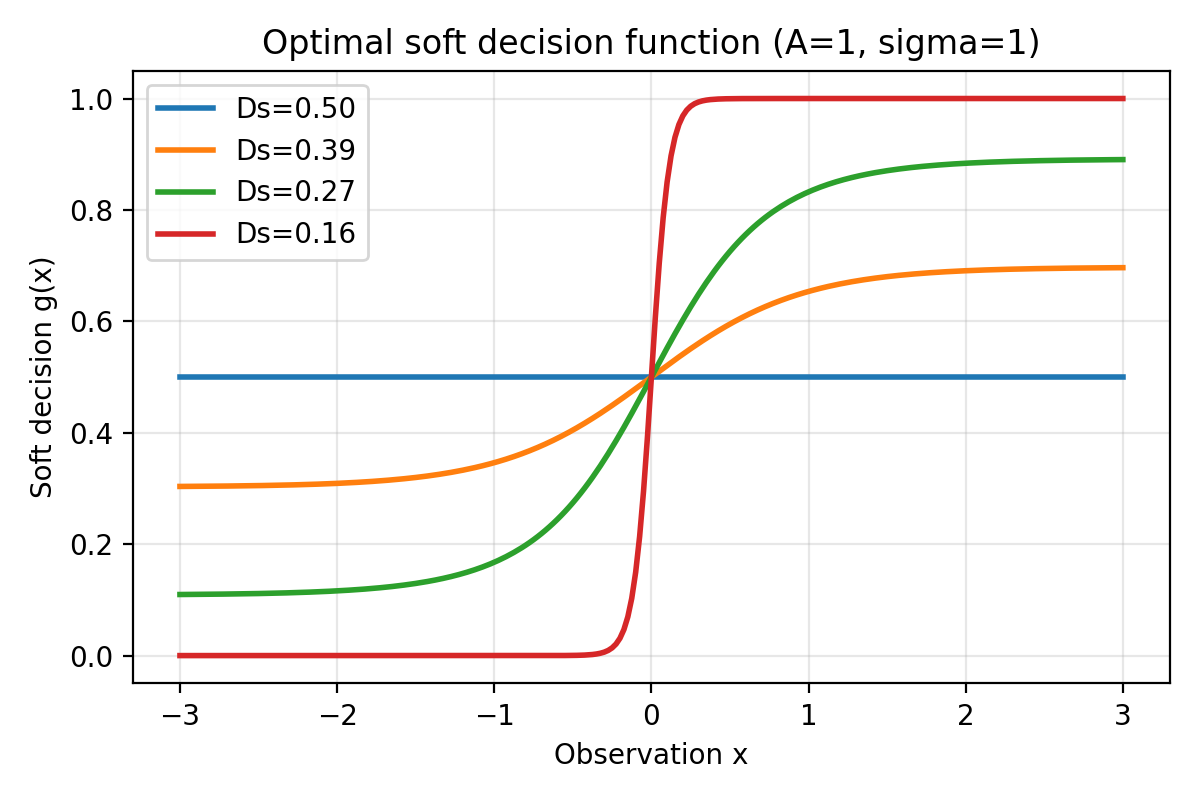
\includegraphics[width=\figw]{../figures/binary_soft_decision_a1_sigma1.png}
\vspace{0.08cm}
\justifying
The soft decision function $g(x)=P(\hat S=0|x)$ becomes sharper when $D_s$ approaches the Bayes error, and flatter as larger semantic distortion is allowed.
\end{block}

\begin{block}{The binary semantic rate decreases as semantic distortion is relaxed}
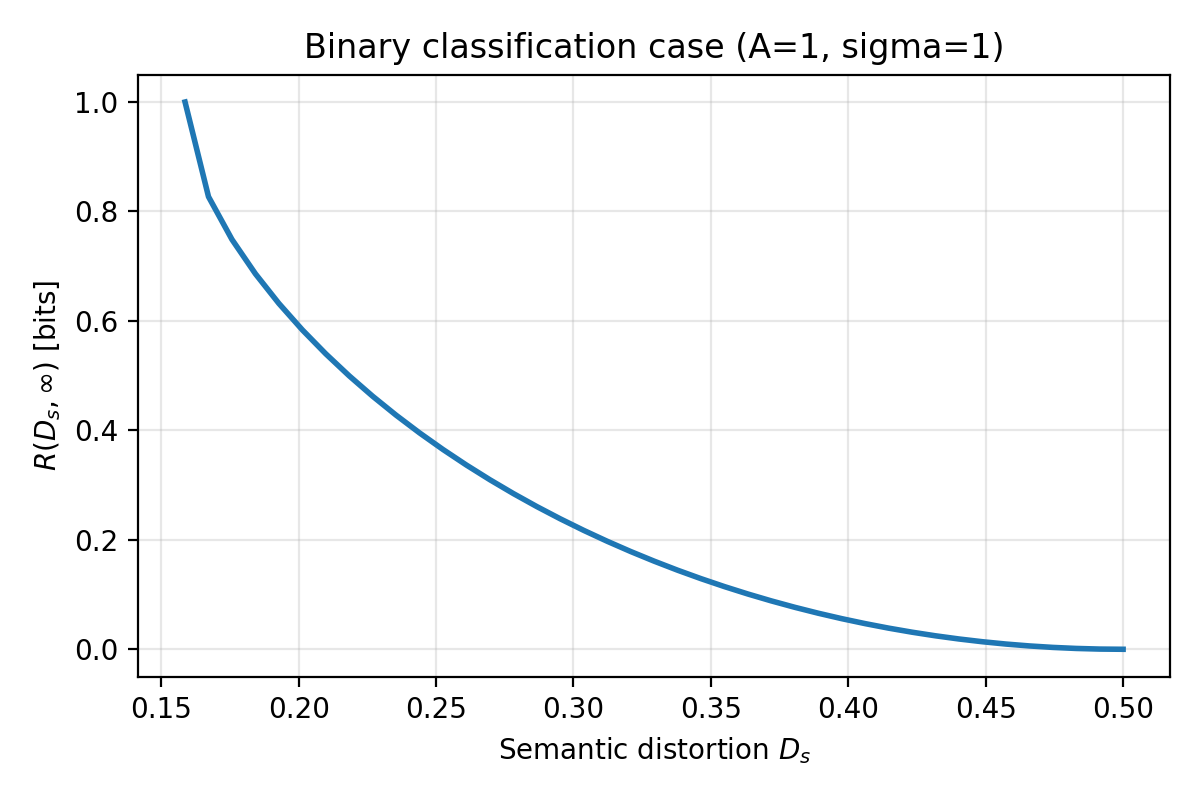
\includegraphics[width=\figw]{../figures/binary_rd_infinite_a1_sigma1.png}
\vspace{0.08cm}
\justifying
Proposition 5 computes $R(D_s,\infty)$ by solving a Lagrange multiplier equation and evaluating an entropy integral over the Gaussian mixture.
\end{block}

\begin{block}{Adding appearance fidelity increases the required rate}
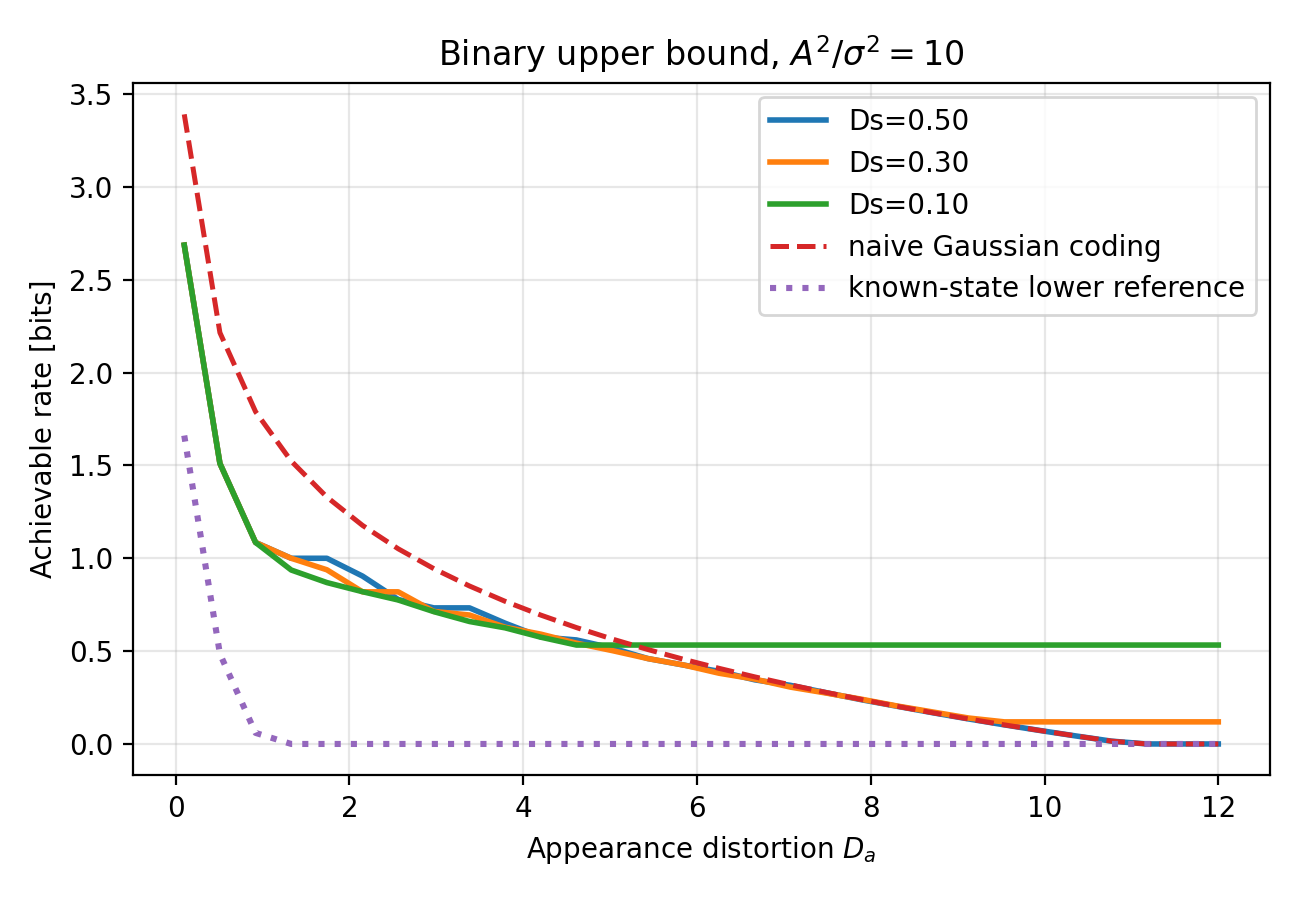
\includegraphics[width=\figw]{../figures/binary_upper_bound_a2sqrt10_sigma1.png}
\vspace{0.08cm}
\justifying
Proposition 6 adds an appearance-refinement term to the semantic rate. Tight $D_a$ constraints require extra bits even when the semantic task is already satisfied.
\end{block}
\end{column}

\begin{column}{0.31\paperwidth}
\begin{block}{Scalar Gaussian sources show an aligned two-constraint maximum}
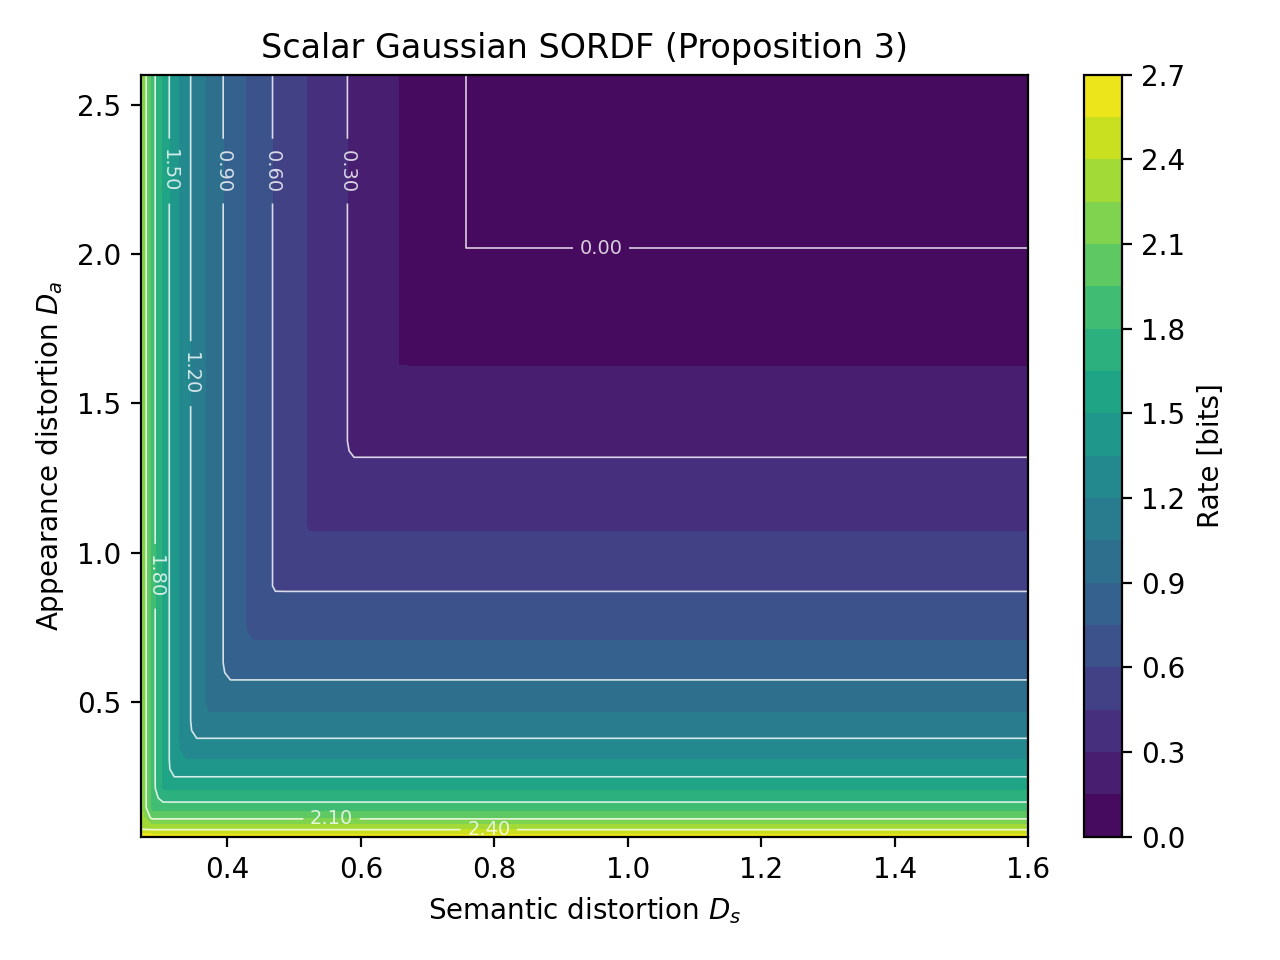
\includegraphics[width=\figw]{../figures/gaussian_scalar_sordf_contour.png}
\vspace{0.08cm}
\justifying
For scalar jointly Gaussian $S$ and $X$, Proposition 3 gives
\[
R=\frac12\max\left\{\log^+\frac{\Sigma_X}{D_a},\;
\log^+\frac{\Sigma_{SX}^2}{\Sigma_X(D_s-\mathrm{mmse})}\right\}.
\]
The larger of the appearance and semantic requirements determines the rate.
\end{block}

\begin{block}{Vector Gaussian sources reveal a genuine semantic--appearance tradeoff region}
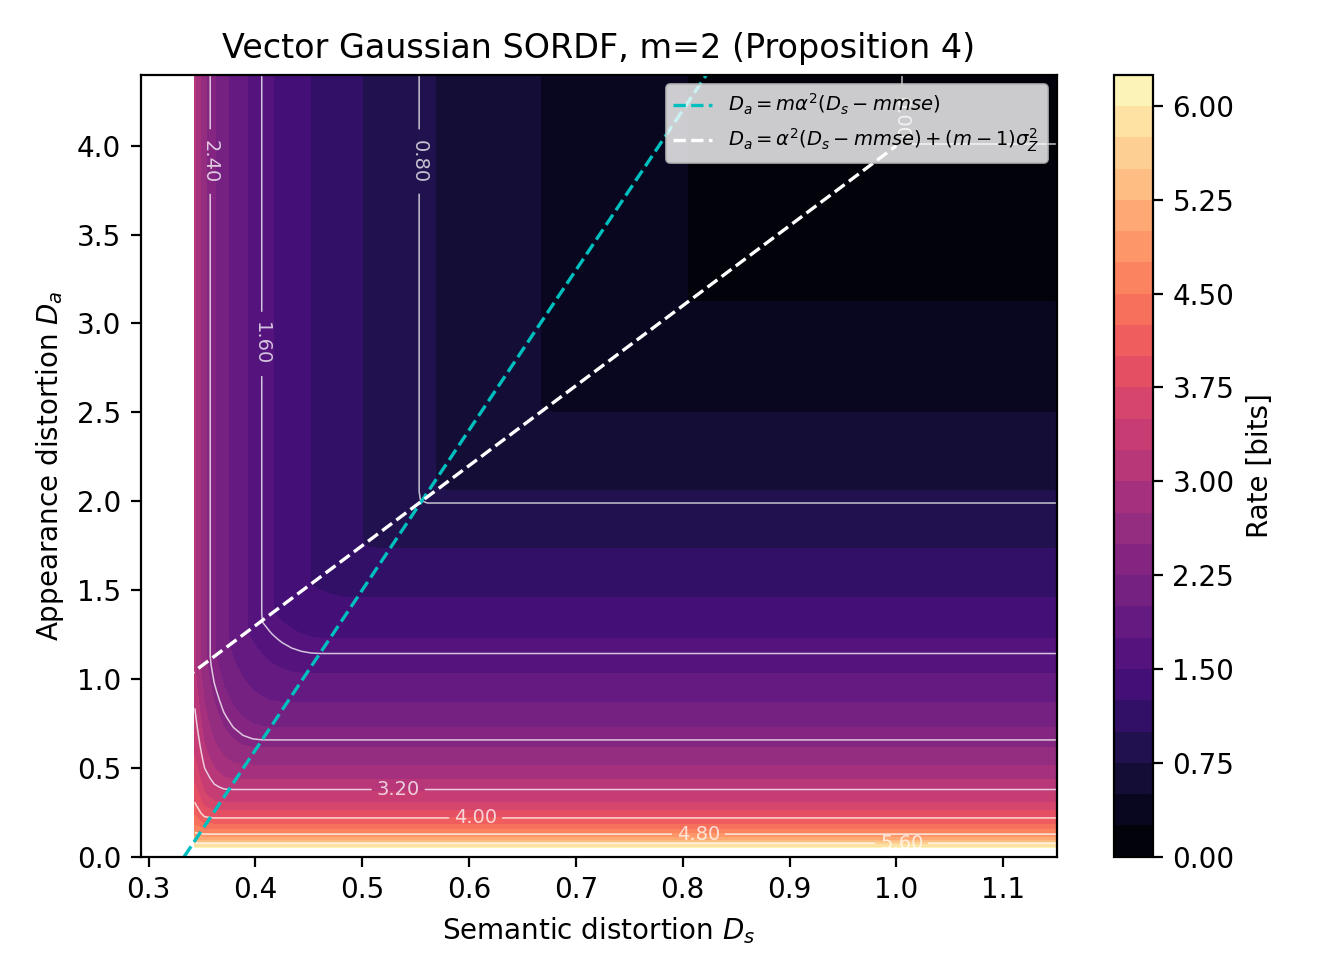
\includegraphics[width=\figw]{../figures/gaussian_vector_sordf_m2_contour.png}
\vspace{0.08cm}
\justifying
For $X=\mathbf 1_m S+Z$, Proposition 4 divides the $(D_s,D_a)$ plane into five regions. The slanted boundaries mark where semantic and appearance constraints interact.
\end{block}

\begin{alertblock}{Takeaways}
\begin{itemize}
  \item Semantic information can be studied using rate--distortion tools.
  \item A hidden state $S$ makes semantic reconstruction an indirect coding problem.
  \item Binary and Gaussian cases expose different tradeoff geometry.
  \item The reproduced figures provide report-ready evidence for the framework.
\end{itemize}
\end{alertblock}
\end{column}

\end{columns}

\vfill
\begin{beamercolorbox}[wd=\paperwidth,sep=0.45cm,center]{headline}
{\small Source paper: Jiakun Liu, Wenyi Zhang, and H. Vincent Poor, ``A Rate-Distortion Framework for Characterizing Semantic Information,'' 2021. Code and generated figures are version controlled in \texttt{rd-semantic-repro}.}
\end{beamercolorbox}

\end{frame}
\end{document}